\graphicspath{{fig/missing/}}

\chapter{Missing data}
\label{cha:missing}

Collecting data of flocking events is a demanding process. Along with the
technical challenges posed by data collection, flocking events are inherently
unpredictable, and so it is not possible to know when and where a flocking
event may occur next. In this way there can become a frustrating
`right-place-right-time' component to data collection.

Typically, recording equipment is set up in a fixed location where the
scientist believes a flocking event may occur. Stationary recording equipment
results in a fixed field of vision in which data may be captured.
Unfortunately, this stationary set-up can result in recording incomplete
flocking events. This may happen when flock members stray outside the field of
vision during a recording event. As the recording equipment is fixed in
location the field of vision cannot be adjusted to reinclude those who move
out-of-frame.

The flock members which move out of frame cannot simply be ignored during
analysis: although we may not observe their movements, they may still be
influencing the behaviour of the observed flock, and so must be accounted for.
Equally undesirable is the temptation to discard all the frames in which any
individual is out of vision, as this has the potential to drastically reduce
the amount of data available for analysis.

In this chapter we will consider how we can handle flocking events which
contain missing observations. Working in a Bayesian framework allows us to
adjust our posterior beliefs about model parameters to account for unobserved
behaviours. We will see that this can be achieved by integrating over all 
possible unobserved trajectories.

\section{Types of missingness}

When we consider flocking events with missing observations, it is important to
consider at which point during the sequence a given agent went missing. This is
because how we handle the missingness will depend on at which point during the
sequence the agent went missing.

Although there are many different circumstances which can result in an agent
leaving our visual field, here we shall consider the two cases which we
consider as the most likely to occur. These two cases arise when agents are
out of frame at the \emph{beginning} of a recording event, or when
agents are out of frame at the \emph{end} of a recording event.

We shall integrate over the possible missing observations using a
Metropolis--Hastings scheme. A proposal mechanism for generating paths missing
at the beginning of a sequence is outlined. Proposed paths can then be accepted
or rejected using results from \cref{cha:sim_studies}. We will then show that
we can generate paths missing at the end of a sequence by implementing a Gibbs
sampler; sampling from our full conditional distributions to realise possible
missing paths.

\subsection{Missing in the beginning}

We say that data is missing at the beginning of a flocking event if the
observer began recording the sequence before all agents had entered the frame.
When we consider this case we assume that all the flock members do eventually
enter the visual field, and so the total number of individuals in the flock is
known.

We imitate this set-up by forward simulating the Vicsek model and imposing a
fixed field of vision on top of the resulting data. We chose to forward
simulate $25$ agents for $40$ time steps. At time $t=1$ agents were directed
and positioned randomly within a square-cell of side length $L=1$. Agents
experienced noise generated from a generalised Student's $t$-distribution with
degrees of freedom $\nu=7$ and scale $\sigma_Y=0.1$. Each individual interacted
with neighbours positioned within distance $r=0.4$, and moved with speed
$\abs{v}=0.03$.

The resulting simulated data is illustrated in \cref{subfig:beg_data}. The
rectangle overlain in black represents our fixed field of vision: analogous to
the fixed visual field generated by recording equipment in the field. The paths
of agents outside this fixed area are classified as missing and are represented
by the red trajectories. Agents move from the positions denoted by the green
markers, to the positions represented by the red makers. It can be seen that
some agents were outside our visual field at the beginning of the simulation.
The ID number of each agent, $i$, is shown at the beginning and end of its
trajectory.

\cref{subfig:beg_missing} shows a schematic representing which data points of
our simulation were considered observed and which data points were classified
as missing. A blue gridpoint in location $(i, t)$ tells us that agent $i$
\emph{was observed} at time $t$. Conversely, a red maker at location $(i, t)$
indicates that agent $i$ \emph{was missing} at time $t$. From this schematic we
can see that a number of agents were missing at time $t=1$: the beginning of
the simulation.

\begin{figure}[tbp]
  \captionsetup[subfigure]{oneside,
                           margin={0.7cm,0cm}}
  \begin{subfigure}[b]{0.5\textwidth}
    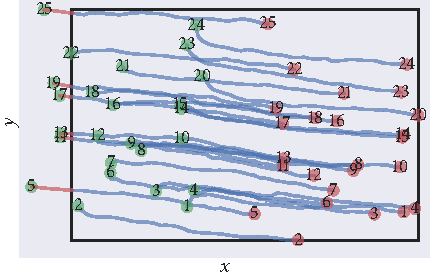
\includegraphics{beg/data.pdf}
    \caption{}
    \label{subfig:beg_data}
  \end{subfigure}%
  \begin{subfigure}[b]{0.5\textwidth}
    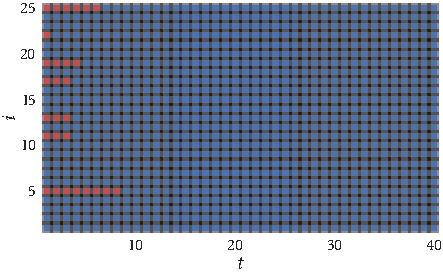
\includegraphics{beg/missing_array.pdf}
    \caption{}
    \label{subfig:beg_missing}
  \end{subfigure}
  \caption{Illustrating our forward simulation of the Vicsek model and the
    data considered missing. \subref{subfig:beg_data} Simulated trajectories.
    The rectangle overlain in black represents our imitation of a fixed
    field of vision: analogous to that of recording equipment used in the
    field. Agents travel from green marker to red marker, with their ID ($i$)
    shown at their start and end points. Data points outside of the rectangular
    region are classified as missing, and are shown by the red trajectories.
    \subref{subfig:beg_missing} Summarising the missing and observed data
    points of our simulation. A blue gridpoint at location $(i, t)$ indicates
    that agent $i$ was within our visual field at time $t$. A red gridpoint at
    location $(i, t)$ indicates that agent $i$ was outside our visual field
    at time $t$.}
  \label{fig:beg_data}
\end{figure}

We may use \cref{eq:likelihood} to quantify the likelihood of observing the
movements of a flock. However, to compute the likelihood we must observe the
positions and directions of each individual in every frame. With this, to
evaluate the likelihood of a flock with missing observations we must be able to
propose candidate values for the missing observations. To do so we shall work
backwards from our first observation of each missing agent.

We propose missing directions of motion backwards in time from our first
observation of each missing agent. A symmetric proposal distribution is used
such that:
\begin{equation}
  \label{eq:propose_beg_dir}
  \theta_{i,t-1}^{\star} \given \nu, \sigma_Y, \theta_{i,t}
    \sim t_{\nu}(\theta_{i,t}, \sigma_Y),
\end{equation}
where $t_{\nu}$ denotes a generalised Student's $t$-distribution with $\nu$
degrees of freedom. An alternative proposal scheme could be formulated using
the interaction term $\angmean{\theta}_{i,t}$ as:
\begin{equation}
  \label{eq:propose_beg_dir_alt}
  \theta_{i,t-1}^{\star} \given \nu, \sigma_Y, \angmean{\theta}_{i,t}
    \sim t_{\nu}(\angmean{\theta}_{i,t}, \sigma_Y).
\end{equation}
However, this proposal mechanism is more computationally expensive than the
proposal scheme outlined in \cref{eq:propose_beg_dir}, as it necessitates the
computation of $\angmean{\theta}_{i,t}$. For highly aligned flocks we expect
\cref{eq:propose_beg_dir,eq:propose_beg_dir_alt} to propose similar candidate
values, with \cref{eq:propose_beg_dir} doing so at a smaller computational
expense. It is for this reason that we shall use the proposal distribution of
\cref{eq:propose_beg_dir}.

Having worked backwards in time to propose plausible values for the unobserved
directions of motion, we can now use these values to realise the corresponding
proposed paths. To do so we rearrange \cref{eq:positional_update} to see:
\begin{equation}
  \label{eq:step_back}
  \bm{x}_{i,t} = \bm{x}_{i,t+1} - \bm{v}_{i,t}.
\end{equation}
Recall from \cref{sec:vicsek_model} that $\bm{v}_{i,t}$ is constructed to have
direction $\theta_{i,t+1}$ and speed $v$. Given $\theta_{i,t+1}$, we may
compute $\bm{v}_{i,t} = (\cos\theta_{i,t+1}, \sin\theta_{i,t+1})^Tv$. With
this, and reindexing $t\mapsto t-1$, we may rewrite \cref{eq:step_back} as:
\begin{equation}
  \label{eq:propose_beg_pos}
  \bm{x}_{i,t-1} = \bm{x}_{i,t} - (\cos\theta_{i,t}, \sin\theta_{i,t})^Tv.
\end{equation}

Having proposed candidate values for the missing directions of motions with
\cref{eq:propose_beg_dir}, we can use \cref{eq:propose_beg_pos} to compute
the proposed paths which these directions correspond to. Now having values for the
positions and directions of motion of every individual at every time step, we
may use \cref{eq:likelihood} to quantify the likelihood of these paths, given
the model parameters.

\subsection{Missing in the end}

\subsection{Missing in the beginning and end}

\section{Simulation studies}

\subsection{Missing in the beginning}

\begin{figure}[tbp]
  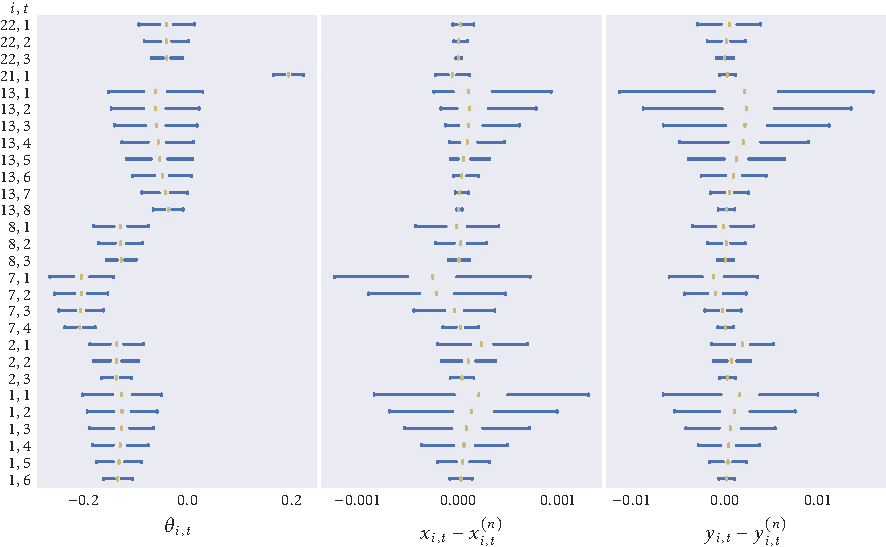
\includegraphics{beg/summary.pdf}
  \caption{caption caption caption}
  \label{fig:beg_summary}
\end{figure}

\begin{figure}[tbp]
  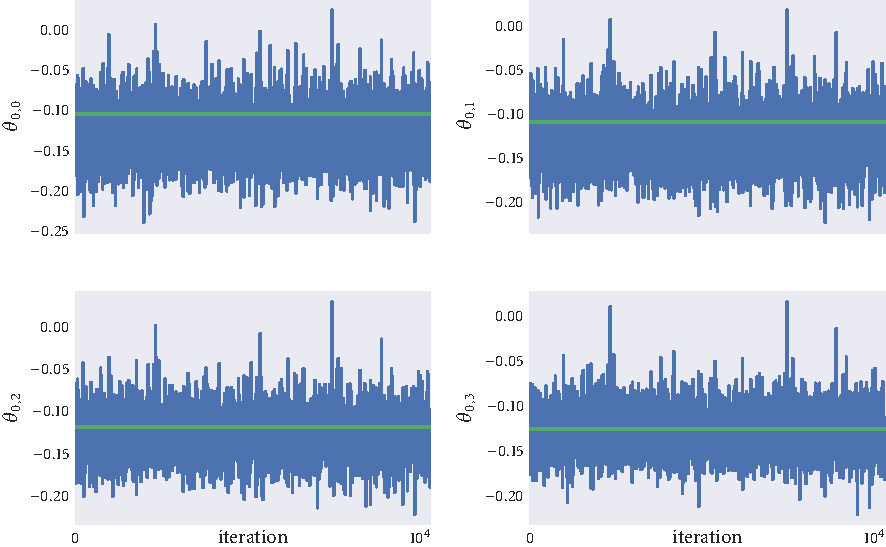
\includegraphics{beg/dir_trace.pdf}
  \caption{}
  \label{fig:beg_dir_trace}
\end{figure}

\begin{figure}[tbp]
  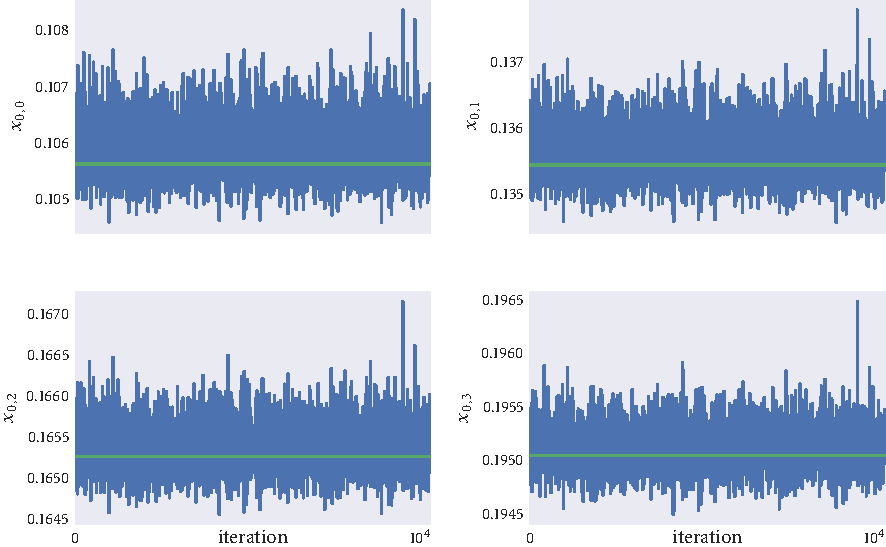
\includegraphics{beg/x_trace.pdf}
  \caption{}
  \label{fig:beg_x_trace}
\end{figure}

\begin{figure}[tbp]
  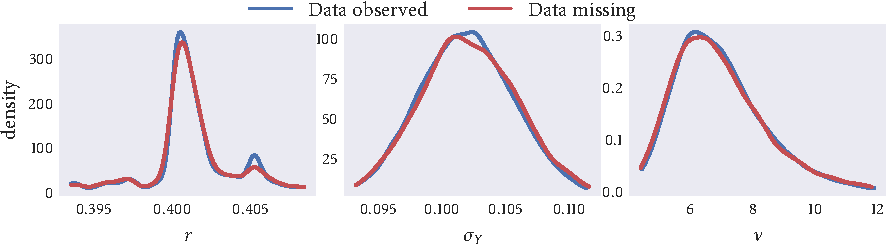
\includegraphics{beg/compare_params.pdf}
  \caption{}
  \label{fig:beg_compare}
\end{figure}


\subsection{Missing in the end}

\subsection{Missing in the beginning and end}

